\chapter{Tilpasning af skalaer}
\label{TestAfSkalaTilpasningAfSkalaer}
%
Som nævnt i \fullref{ParametreDelKonklusion} er skalaerne udviklet specifikt til ét enkelt parameter, hvorfor der ikke er taget højde for helhedsindtrykket. Det vil derfor i følgende afsnit fokuseres på at videreudvikle og tilpasse skalaerne, blandt andet i forhold til at opnå en form for konsistens relateret til formuleringen af skala spørgsmål, labels samt skalatype. Målet er ikke at alle skalaer er ens, men at tilpasse skalaerne så de fremstår mere præsentable end hvad tilfældet er nu, samt at samle de skalaer, hvis skala spørgsmål stilles på samme måde. Derudover tilstræbes det, at gruppere skalaerne efter det emne de evaluerer. For at undgå at testpersonerne angiver det samme punkt på skalaerne, fordi to parametre vedrører det samme emne, vil det tilstræbes ikke at placerer skalaerne lige efter hinanden, hvis de vedrører det samme emne. Det forventes, at ved at tilpasse og videreudvikle skalaerne vil det være lettere for testpersonerne at evaluerer interaktionen med robotten. Der tages udgangspunkt i de udvalgte skalaer, der blev præsenteret i \fullref{ParametreDatabehandlingSkalaer}.

Foruden at tilpasse og videreudvikle de udvalgte skalaer vil der ligeledes fokuseres på at vælge den rækkefølge, hvorved skalaerne efterfølgende skal præsenteres for testpersonerne.    
%
\section{Tilpasning og rækkefølge på skalaer}
\label{TilpasningSkalaer}
%
En af årsagerne til at skala spørgsmål eller labels omformuleres og en anden skalatype vælges er, at risikoen for potentiel bias ved at lægge ord i munden på testpersonerne mindskes. En anden årsag er, at der er situationer, hvor det valgte spørgsmål og de valgte labels ikke passer sammen i forhold til at fuldende en sætning og situationer, hvor spørgsmål og label modsiger hinanden. Da der tilstræbes en form for konsistens, i forhold til helhedsindtrykket, vil skalaerne ydermere blive vurderet i forhold til hvordan de passer sammen, for på den måde at gruppere skalaer, der er formuleret og præsenteret ens. 

Der vil foretages nogle grafiske ændringer på skalaerne, såsom at centrere skala spørgsmålet over skalaen, i modsætning til skalaerne præsenteret i \fullref{ParametreDatabehandlingSkalaer}, hvor skala spørgsmålet stod til venstre. I tillæg vil grammatiske fejl blive rettet. Når skalaerne præsenteres for testpersonerne, vil testpersonerne maksimalt få præsenteret fire skalaer af gangen. Det skyldes, at skalaerne præsenteres på en \textit{Microsoft Surface Pro (5)}, hvis skærm er 12.3" med en opløsning på 2736 x 1824. Det besluttes at der kun er plads til fire skalaer, da skalaerne ellers vil være for kompakte. I \fullref{TestAfSkalaProgramSkala} vil den praktiske del af opsætningen af skalaerne blive uddybet. \blankline 
%
Den første skala, der præsenteres for testpersonerne vedrører hvordan robottens skærm reagerede, jævnfør \autoref{fig:TilpasningSkaermensReaktion}. Det vælges at dette skala spørgsmål skal præsenteres først, hver gang, da testpersonerne responderer på skalaerne på en anden skærm, som reagerer på en anden måde. Ved at præsentere dette skala spørgsmål først vil skærmens reaktionsevne på robotten være frisk i hukommelsen, og testpersonerne vil derfor have mindre at sammenligne med i forhold til reaktionsevne på skærmen, hvor skalaerne præsenteres. Da testpersonerne interagerer med to skærme; robottens og computeren hvorpå skalaerne præsenteres, vælges det at omformulere skala spørgsmålet så det specificeres, hvilken skærm testpersonen skal evaluere.  
%
%DE FIRE FØLGENDE SKALAER HØRER TIL DEN SAMME GRUPPE OG SKAL PRÆSENTERES PÅ DEN SAMME SKÆRM.
%
\begin{figure}[H]
\centering
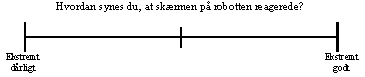
\includegraphics[width =\textwidth]{Figure/TilpasningAfSkalaer/TilpassetSkaermensReaktion} 
\caption{Tilpasset skala til: \textit{Hvordan synes du skærmen på robotten reagerede?}.}
\label{fig:TilpasningSkaermensReaktion}
\end{figure}
\noindent
%
Det vælges at omformulere skala spørgsmålet: \textit{Jeg synes at robotten er imødekommende} af to årsager: 1) At bruge ordet \textit{imødekommende} i den sætning er ledende, hvorfor det potentielt kan være en bias for testpersonerne, og 2) Formuleringen i spørgsmålet passer ikke med de valgte labels i forhold til at fuldende en sætning. Det giver ikke mening at stille spørgsmålet: \textit{Jeg synes at robotten er imødekommende} og så have en svarmulighed, der hedder: \textit{Ekstremt afvisende}. Årsagen til at skalaen ikke præsenteres på samme måde som de skalaer, der tilhører: \textit{Hvad synes du om robotten?} er, at fælles for de skalaer er, at de præsenteres på en unipolær skala. Hvis dette skala spørgsmål skulle præsenteres på en unipolær skala, ville det være nødvendigt at danne to skalaer - én til \textit{afvisende} og én til \textit{imødekommende}. Af de årsager vælges det at omformulere skala spørgsmålet til: \textit{Hvordan oplevede du robotten?}, hvor tidligere valgte labels bibeholdes, jævnfør \autoref{fig:TilpasningOplevede}.
%
\begin{figure}[H]
\centering
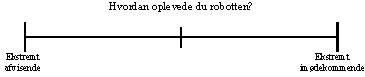
\includegraphics[width =\textwidth]{Figure/TilpasningAfSkalaer/TilpassetOplevede} 
\caption{Tilpasset skala til: \textit{Hvordan oplevede du robotten?}.}
\label{fig:TilpasningOplevede}
\end{figure}
\noindent
%
I henhold til skalaen gengivet på \autoref{fig:TilpasningBrugAfR}, foretages der ingen ændringer i forhold til den udvalgte skala. Det vælges, at placere skalaen efter \textit{Hvordan oplevede du robotten}, jævnfør \autoref{fig:TilpasningOplevede}, fordi dette skala spørgsmål dels er formuleret på samme måde og dels fordi det hænger sammen med det første skala spørgsmål: \textit{Hvordan synes du, at skærmen på robotten reagerede?}.
%
\begin{figure}[H]
\centering
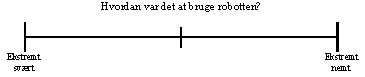
\includegraphics[width =\textwidth]{Figure/TilpasningAfSkalaer/TilpassetHvordanVarDetAtBrugeR} 
\caption{Tilpasset skala til: \textit{Hvordan var det at bruge robotten?}.}
\label{fig:TilpasningBrugAfR}
\end{figure}
\noindent
%
Skala spørgsmålet: \textit{Jeg synes at robottens bevægelser er} omformuleres, fordi skalaens labels: \textit{Ekstremt rolige} og \textit{Ekstremt vilde}, ikke passer sammen med de labels, som er på skalerne, hvis skala spørgsmål egentlig passer med \textit{Jeg synes at robottens bevægelser er} såsom: \textit{Jeg synes at robottens hastighed er}, hvis labels er: \textit{Alt for langsom}, \textit{Fin} og \textit{Alt for hurtig}, for henholdvist venstre, midtpunkt og højre label. Af den årsag vælges det er omformulere skala spørgsmålet til: \textit{Hvordan oplevede du robottens bevægelser?}, jævnfør \autoref{fig:TilpasningBevaegelserR}. Da denne formulering passer godt med: \textit{Hvordan oplevede du robotten?} vælges det, at præsentere denne skala, som den fjerde skala. 
%
\begin{figure}[H]
\centering
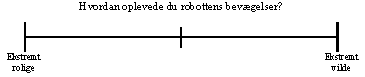
\includegraphics[width =\textwidth]{Figure/TilpasningAfSkalaer/TilpassetBevaegelserR} 
\caption{Tilpasset skala til: \textit{Hvordan oplevede du robottens bevægelser?}.}
\label{fig:TilpasningBevaegelserR}
\end{figure}
\noindent
%
%DE TRE FØLGENDE SKALAER HØRER TIL DEN SAMME GRUPPE OG SKAL PRÆSENTERES PÅ DEN SAMME SKÆRM.
De følgende tre skalaer for henholdvis robottens afstand \autoref{fig:TilpasningRStoppede}, hastighed \autoref{fig:TilpasningHastighedR}, og højde \autoref{fig:TilpasningHoejdeR}, vil blive præsenteret sammen, både fordi de minder om hinanden og fordi de alle tre er fysiske parametre. De tre skala spørgsmål, labels og skalatype er stort set ens med den ene undtagelse, at der til skala spørgsmålet: \textit{Jeg synes, at robotten stoppede...}, ikke har et label på midtpunktet. De eneste ændringer, der er foretaget på de tre skalaer i forhold til dem, som blev præsenteret i \fullref{ParametreDatabehandlingSkalaer} er, at spørgsmålet er centreret, der er tilføjet tre punktummer efter spørgsmålet, og sat et komma efter \textit{synes}.
%
\begin{figure}[H]
\centering
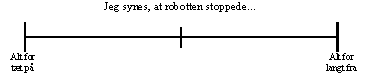
\includegraphics[width =\textwidth]{Figure/TilpasningAfSkalaer/TilpassetRStoppede} 
\caption{Tilpasset skala til: \textit{Jeg synes, at robotten stoppede...}.}
\label{fig:TilpasningRStoppede}
\end{figure}
\noindent
%
%
\begin{figure}[H]
\centering
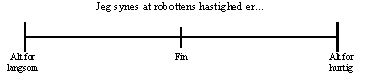
\includegraphics[width =\textwidth]{Figure/TilpasningAfSkalaer/TilpassetHastighedR} 
\caption{Tilpasset skala til: \textit{Jeg synes, at robottens hastighed er...}.}
\label{fig:TilpasningHastighedR}
\end{figure}
\noindent
%
%
\begin{figure}[H]
\centering
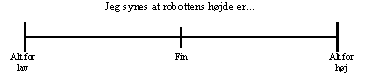
\includegraphics[width =\textwidth]{Figure/TilpasningAfSkalaer/TilpassetHoejdeR} 
\caption{Tilpasset skala til: \textit{Jeg synes, at robottens højde er...}.}
\label{fig:TilpasningHoejdeR}
\end{figure}
\noindent
%
%DE SEKS FØLGENDE SKALAER HØRER TIL DEN SAMME GRUPPE OG SKAL PRÆSENTERES PÅ TO SKÆRME.
Da nogle af de udvalgte skalaer i forvejen er formuleret som udsagn testpersonerne kan erklære sig helt uenige eller helt enige i, vælges det at præsentere disse skalaer sammen og på ens skalaer. Den første skala, der vil blive præsenteret i det henseende er til skala spørgsmålet: \textit{Jeg føler, at robotten kan hjælpe mig}, jævnfør \autoref{fig:TilpasningRobottenKanHjaelpe}. I forhold til udvælgelsen vil skalaen fremover blive præsenteret uden et navngivet label på midtpunktet. 
%
\begin{figure}[H]
\centering
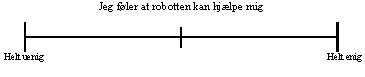
\includegraphics[width =\textwidth]{Figure/TilpasningAfSkalaer/TilpassetRobottenKanHjaelpe} 
\caption{Tilpasset skala til: \textit{Jeg føler, at robotten kan hjælpe mig}.}
\label{fig:TilpasningRobottenKanHjaelpe}
\end{figure}
\noindent
% 
Skalaen hvorpå \textit{Jeg synes, at robotten stod i vejen} evalueres får både tildelt nye labels og ny skalatype, jævnfør \autoref{fig:TilpasningRobottenErIVejen}. Årsagen til det er, at de labels, der var tildelt: \textit{Slet ikke i vejen} og \textit{Ekstremt i vejen} ikke passer særligt godt til at fuldende sætningen med skala spørgsmålet og fordi det antages, at der kan opstå bias mellem spørgsmål og label, som de formuleret nu. Det vælges derfor at præsentere skalaen som en bipolær skala, hvor testpersonerne angiver, hvor helt uenige eller helt enige de er i, at robotten stod i vejen.
%
\begin{figure}[H]
\centering
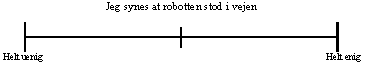
\includegraphics[width =\textwidth]{Figure/TilpasningAfSkalaer/TilpassetRobottenErIVejen} 
\caption{Tilpasset skala til: \textit{Jeg synes, at robotten er i vejen}.}
\label{fig:TilpasningRobottenErIVejen}
\end{figure}
\noindent
%
I henhold til de to labels: \textit{Ekstremt utryg} og \textit{Ekstremt tryg}, der er anvendt på skalaen til \textit{Jeg føler mig utryg ved robotten}, er det klart, at der ikke forekommer særlig god overenstemmelse mellem label og spørgsmål, når sætningen fuldendes. Af den årsag og for at undgå at lægge ord i munden på testpersonerne, vælges det at omformulere de to labels, så skalaen går fra: \textit{Helt uenig} til \textit{Helt enig}, jævnfør \autoref{fig:TilpasningTrygVedR}.
%
\begin{figure}[H]
\centering
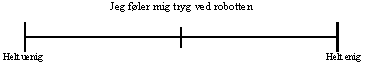
\includegraphics[width =\textwidth]{Figure/TilpasningAfSkalaer/TilpassetTrygVedR} 
\caption{Tilpasset skala til: \textit{Jeg føler mig tryg ved robotten}.}
\label{fig:TilpasningTrygVedR}
\end{figure}
\noindent
%
De følgende tre skalaer hænger egentlig sammen med de tre foregående skalaer, men da det er valgt maksimalt at præsenterer fire skalaer på en side, vælges det at præsentere de seks skalaer på to sider med tre skalaer på hver. 

Igen opleves der uoverensstemmelse mellem labels: \textit{Slet ikke forskrækket} og \textit{Ekstremt forskrækket}, og skala spørgsmålet: \textit{Robotten gjorde mig forskrækket}. Det vælges derfor at ændre skalaen fra en unipolær til en bipolær skala, hvorpå testpersonerne kan angive hvor helt uenige eller helt enige de er i, at robotten forskrækkede dem, jævnfør \autoref{fig:TilpasningForskraekket}.
%
\begin{figure}[H]
\centering
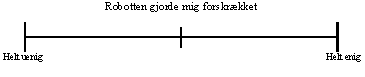
\includegraphics[width =\textwidth]{Figure/TilpasningAfSkalaer/TilpassetForskraekket} 
\caption{Tilpasset skala til: \textit{Robotten gjorde mig forskrækket}.}
\label{fig:TilpasningForskraekket}
\end{figure}
\noindent
% 
Tilsvarene uoverensstemmelse gør sig gældende for skala spørgsmålet: \textit{Jeg kan godt lide at blive betjent af robotten}, hvis endepunkter er navngivet med henholdvis: \textit{Slet ikke} og \textit{Ekstremt meget}. Det vælges at bibeholde formuleringen af skala spørgsmålet og ændre skalatypen fra en unipolær skala til en bipolær skala med et midtpunkt. Dertil vælges det, at testpersonerne evaluerer skala spørgsmålet i forhold til hvor helt uenige eller helt enige de er, jævnfør \autoref{fig:TilpasningLideBetjening}.   
%
\begin{figure}[H]
\centering
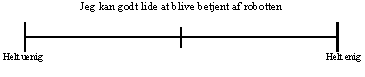
\includegraphics[width =\textwidth]{Figure/TilpasningAfSkalaer/TilpassetLideBetjening} 
\caption{Tilpasset skala til: \textit{Jeg kan godt lide at blive betjent af robotten}.}
\label{fig:TilpasningLideBetjening}
\end{figure}
\noindent
% 
De eneste ændringer, der er foretaget i forbindelse med skalaen til: \textit{Jeg regnede med, at robotten fulgte mig hen til det sted jeg valgte} er det grafiske med centreringen af skala spørgsmålet, en kommarettelse samt fjernelse af midtpunktets label: \textit{Neutral}, jævnfør \autoref{fig:TilpasningRobottenFulgte}.
%
\begin{figure}[H]
\centering
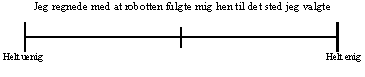
\includegraphics[width =\textwidth]{Figure/TilpasningAfSkalaer/TilpassetRobottenFulgteMigDetRigtigeStedHen} 
\caption{Tilpasset skala til: \textit{Jeg regnede med at robotten fulgte mig hen til det sted jeg valgte}.}
\label{fig:TilpasningRobottenFulgte}
\end{figure}
\noindent
%
Selvom der er seks skala, hvorpå testpersonerne kan erklærer sig helt uenige eller helt enig i skala spørgsmålet er det valgt, at præsentere de tre første på én side og de tre næste på den næste side. Rækkefølgen er valgt efter, at \textit{Jeg føler, at robotten kan hjælpe mig} og \textit{Jeg regnede med, at robotten fulgte mig hen til det sted jeg valgte} minder om hinanden, hvorfor de to skalaer præsenteres på hver sin side. I tillæg minder \textit{Jeg kan godt lide at blive betjent af robotten} i højere grad om \textit{Jeg føler, at robotten kan hjælpe mig} end om \textit{Jeg regnede med, at robotten fulgte mig hen til det sted jeg valgte}, hvorfor det vurderes at dette skala spørgsmål kan præsenteres på samme side som sidstnævnte. Derudover vælges det at præsentere: \textit{Jeg føler mig tryg ved robotten} og \textit{Robotten gjorde mig forskrækket} på hver sin side, da de muligvis hænger sammen. \blankline
%
%DE TO FØLGENDE SKALAER HØRER TIL DEN SAMME GRUPPE OG SKAL PRÆSENTERES PÅ DEN SAMME SKÆRM.
Det vælges at omformulere skala spørgsmålet: \textit{Jeg oplever robottens hjælp som personlig}, dels for at undgå at lægge ord i munden på testpersonerne og fordi det ved den formulering antages at testpersonerne har oplevet robottens hjælp som personlig. Derudover er det ikke muligt med de to labels: \textit{Slet ikke personlig} og \textit{Ekstremt personlig}, at fuldende sætningen efter spørgsmålet. Det vælges derfor at omformulere skala spørgsmålet til: \textit{Hvor personlig oplevede du robottens hjælp?} og bibeholde de to labels, jævnfør \autoref{fig:TilpasningPersonligHjaelp}. 
%
\begin{figure}[H]
\centering
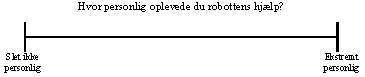
\includegraphics[width =\textwidth]{Figure/TilpasningAfSkalaer/TilpassetPersonligHjaelp} 
\caption{Tilpasset skala til: \textit{Hvor personlig oplevede du robottens hjælp?}.}
\label{fig:TilpasningPersonligHjaelp}
\end{figure}
\noindent
%
Af samme årsag omformuleres skala spørgsmålet: \textit{Jeg blev overrasket over robottens henvendelse} til \textit{Hvor overrasket blev du over robottens henvendelse?}, hvor de to labels bibeholdes, jævnfør \autoref{fig:TilpasningOverrasketOverR}. 
%
\begin{figure}[H]
\centering
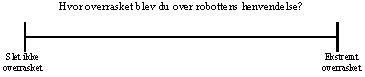
\includegraphics[width =\textwidth]{Figure/TilpasningAfSkalaer/TilpassetOverrasketOverR} 
\caption{Tilpasset skala til: \textit{Hvor overrasket blev du over robottens henvendelse?}.}
\label{fig:TilpasningOverrasketOverR}
\end{figure}
\noindent
%  
De resterende udvalgte skalaer, som har det til fælles, at deres skala spørgsmål er formuleret: \textit{Jeg synes at robotten er} efterfulgt af en parameter, vil alle høre under ét samlet skala spørgsmål: \textit{Hvad synes du om robotten?}, jævnfør \autoref{fig:TilpasningHvadSynesDuOmR}. Årsagen er blandt andet, at det for de enkelte skala spørgsmål ikke var muligt at fuldende sætningerne med de angivne labels, og derudover vurderes det, at hvis parameteren, som testpersonen skal evaluere, står i skala spørgsmålet er der risiko for at der opstår bias, når samme parameter står i begge labels. Grunden til at det overhovedet blev besluttet at sammensætte denne type skala spørgsmål til ét skala spørgsmål, med otte tilhørende skalaer, var skala spørgsmålet: \textit{Jeg synes, at robotten er imødekommende}. Problemet med det skala spørgsmål i forhold til de resterende skalaer, vedrørerende testpersonernes mening om robotten, er, at skalaen er bipolær. Med en bipolær skala fra \textit{Ekstremt afvisende} til \textit{Ekstremt imødekommende} kan det potentielt medføre, at det kun er den ene halvdel af skalaen, der bliver brugt så længe skala spørgsmålet indeholder ordet: \textit{imødekommende}. 

Da det er besluttet, at der maksimalt må præsenteres fire skala på skærmen af gangen er det nødvendigt, at fordele de otte skalaer i to. Ligesom tidligere vil to skalaer, der formentlig vedrører det samme emne, blive præsenteret på hver sin side. Med udgangspunkt på i det vil skalaerne med parameterne: \textit{Irriterende} og \textit{anmassende} blive præsenteret på hver sin side, hvor førstnævnte præsenteres på den første af de to sider. Det vælges at parameterne: \textit{Elegant} og \textit{sød} præsenteres på den første side, dog ikke efter hinanden, hvor \textit{sej} og \textit{sjov} præsenteres på den anden side. Grunden til at de fire parametre er fordelt på denne måde er, at det forventes, at særligt \textit{sød}, \textit{sjov} og \textit{sej} formentlig måler det samme, hvor det i mindre grad forventes at \textit{sød} og \textit{elegant} måler det samme. Dertil er skalaen for parameteren \textit{spændende} placeret mellem \textit{elegant} og \textit{sød} for at indikere, at der er forskel mellem de to parametre. Det samme er gældende for \textit{sej} og \textit{sjov}, som er adskildt med \textit{anmassende}. Rækkefølgen på de otte skalaer fremgår af \autoref{fig:TilpasningHvadSynesDuOmR}.
\newpage
%
\begin{figure}[H]
\centering
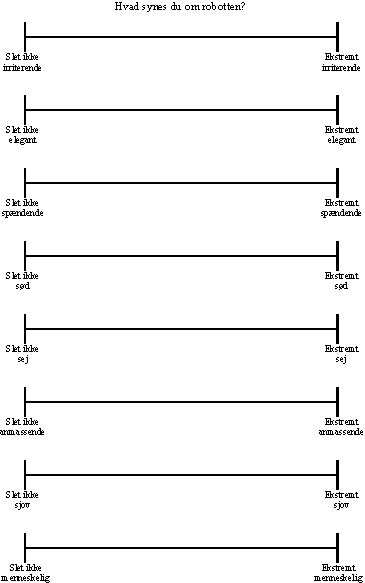
\includegraphics[width =\textwidth]{Figure/TilpasningAfSkalaer/HvadSynesDuOmR} 
\caption{Tilpasset skalaer til: \textit{Hvad synes du om robotten}.}
\label{fig:TilpasningHvadSynesDuOmR}
\end{figure}
\noindent
%
Som tidligere nævnt vil skala spørgsmålet: \textit{Hvor meget kendskab har du til teknologi/robotter?} ikke blive behandlet på samme måde som de resterende parametre, da det vil indgå som en del af demografi indsamlingen, hvorfor det ikke vil blive beskrevet yderligere i dette afsnit. 


